\documentclass[a4paper]{article}

%% Language and font encodings
\usepackage[english]{babel}
\usepackage[utf8x]{inputenc}
\usepackage[T1]{fontenc}

%% Sets page size and margins
\usepackage[a4paper,top=3cm,bottom=2cm,left=3cm,right=3cm,marginparwidth=1.75cm]{geometry}

%% Useful packages
\usepackage{amsmath}
\usepackage{amsfonts}
\usepackage{graphicx}
\usepackage{subcaption}
\usepackage[colorinlistoftodos]{todonotes}
\usepackage[colorlinks=true, allcolors=blue]{hyperref}

\graphicspath{ {figures/} }

\title{Possible Inconsistency in Maximum Likelihood Calculation of Ancestral States}
\author{Shaw, Matsen, Minin}

\begin{document}
\maketitle

%comments from Erick:
% >  This is great!
% > - would be great to have all the calculations showing the "refinement" structure written out for the various tree structures (just done by hand and scanned is just fine)
% > - I think of the "refinement" as a partition, so perhaps rather than "empty refinement" we have a "single-element partition"
% > - in order to interpret the site patterns I need to figure out in what order the leaves are labeled
% > - how is ell calculated?
% > - on the numerical sanity check, it doesn't seem clear that the branch lengths can be different than the inferred ones-- they can!
% > - re "general case", agreed though I don't think that we need numerical optimization of branch lengths in a set of a branch length partition-- we can just get the optimal branch length directly. Namely, for each branch, we know all hidden states (given that we are in a set of a partition) and so can count the number of mutations across that branch. From there we have a simple likelihood function, which either has an optimal in the interior or on the boundary of the partition.

\renewcommand{\arraystretch}{1.2} % because otherwise exponents get eaten by \hline


\section*{Introduction}

Classical maximum-likelihood (ML) estimation in phylogenetics operates by integrating out possible ancestral states at the internal nodes of the tree.
Recently \cite{Neher2017} have suggested using an approximation to ML inference in which the likelihood is maximized jointly across model parameters and ancestral sequences.
This is attractive from a computational perspective: joint ML inference can proceed according to an iterative procedure in which ML ancestral sequences are first inferred and then model parameters are optimized conditional on the ancestral sequences.
% I would say classical maximum likelihood is closer to EM, no? At some point in EM we'd have to marginalize/take the expectation, which joint ML doesn't do. Curious to talk more about it though...
This latter step is much simpler and more computationally efficient when conditioning on ancestral sequences compared to the case in which ancestral sequences are marginalized out.

However, existing consistency proofs for phylogenetics \cite{ArindamRoyChoudhury?} do not apply to the setting of joint inference of trees and ancestral sequences, raising the question of whether this procedure enjoys good statistical properties.
There are examples in statistics, such as the Neyman-Scott paradox \cite{Neyman1948-tt}, in which additional parameters destroy consistency.

In this paper we show that the joint inference of trees and ancestral sequences is not consistent in general.
To do so, we follow a strategy of using simple models and four taxa trees.
Here we use a binary symmetric model and simulate on the ``Farris zone'' \cite{Siddall1998-hq} tree.
We use bounds on the joint likelihood to demarcate a sizeable area of long branch lengths in which joint inference converges on the wrong tree.

\section{Ancestral state reconstruction using maximum likelihood}

\subsection{Classical maximum-likelihood inference in phylogenetics}

We observe character data $\mathbf{y}=[y_1,\ldots,y_n]\in\mathcal{Y}^n$ and corresponding unknown ancestral states $\boldsymbol\xi=[\xi_1,\ldots,\xi_n]\in\Xi^n$.
Both $\mathcal{Y}$ and $\Xi$ are discrete sets.
Without loss of generality, assume $\mathcal{Y}=\Xi=\{0,1\}$.
For a topology $\tau$ and branch lengths $t$ we form the likelihood
\begin{equation}
\label{eq:full_likelihood}
L_n(\mathbf{y};\boldsymbol\xi, \tau, t) = \prod_{i=1}^{n} \ P(y_i, \xi_i | \tau, t).
\end{equation}
In particular, we are interested in
$$
(\hat{\boldsymbol\xi}, \hat{\tau}, \hat{t}) = \arg\max_{\boldsymbol\xi, \tau, t} \ L_n(\mathbf{y};\boldsymbol\xi, \tau, t),
$$
which we call the maximum likelihood values of the parameters $(\boldsymbol\xi, \tau, t)$.

Since the number of elements in $\boldsymbol\xi$ grows with that of the observed data $\mathbf{y}$, the typical approach to estimate these parameters involves computing the marginal likelihood
\begin{equation}
\label{eq:marginal_likelihood}
\tilde{L}_n(\mathbf{y}; \tau, t) = \sum_{\boldsymbol\xi} \ L_n(\mathbf{y};\boldsymbol\xi, \tau, t).
\end{equation}
and maximizing over the topology and branch lengths to obtain
$$
(\hat{\tau}, \hat{t}) = \arg\max_{\tau, t} \  \tilde{L}_n(\mathbf{y}; \tau, t).
$$
The values $\hat{\boldsymbol\xi}$ are then calculated conditional on these estimates.
More likely in practice we fix a topology $\tau$ and use this marginalization approach to compute $(\hat{\boldsymbol\xi}, \hat{t})$.

\subsection{Joint maximization}

One tantalizing approach is to do away with the marginalization and the two-step maximization, directly estimating the maximum likelihood parameters from the full likelihood in \eqref{eq:full_likelihood}.
We can perform this by computing the profile likelihood
\begin{equation}
\label{eq:profile_likelihood}
L_n'(\mathbf{y};\tau, t) = \max_{\boldsymbol\xi} \ L_n(\mathbf{y};\boldsymbol\xi, \tau, t),
\end{equation}
then estimating the topology and branch lengths via
\begin{equation}
\label{eq:profile_likelihood_topology_bl}
(\hat{\tau}, \hat{t}) = \arg\max_{\tau, t} \ L_n'(\mathbf{y};\tau, t)
\end{equation}
while using $\hat{\boldsymbol\xi}$ from \eqref{eq:profile_likelihood} as an estimate for $\boldsymbol\xi$.
Since $\Xi$ is a discrete set, there exists a maximum \eqref{eq:profile_likelihood}, and so \eqref{eq:profile_likelihood_topology_bl} will recover the joint ML values of the unknown parameters.
In the general case, the functional form of \eqref{eq:profile_likelihood} is determined by inequalities that depend on the unknown $(\tau,t)$.
For this reason, in practice joint ML estimates $\hat{\boldsymbol\xi}$ for a fixed $(\tau,t)$, then $(\hat{\tau},\hat{t})$ given $\hat{\boldsymbol\xi}$, maximizing each of these conditional objectives until convergence \cite{Neher2017}.

\subsection{Site pattern formulation}

Since $\mathcal{Y}$ and $\Xi$ are discrete sets, we define unique site patterns $\mathbf{s}=[s_1,\ldots,s_q]\in\mathcal{S}$ and ancestral state patterns $\mathbf{z}=[z_1,\ldots,z_q]\in\mathcal{Z}$ such that
\begin{align}
L_n'(\mathbf{y};\tau, t) &= \max_{\boldsymbol\xi} \ L_n(\mathbf{y};\boldsymbol\xi, \tau, t) \\
    &= \max_{\boldsymbol\xi} \ \prod_{i=1}^{n} \ P(y_i, \xi_i | \tau, t) \\
    &= \max_{\mathbf{z}} \ \prod_{j=1}^{q} \ P(s_j, z_j | \tau, t)^{n_j} \label{eq:site_pattern_likelihood}
\end{align}
where $n_j$ is the number of observations in the sample where site pattern $s_j$ was seen.
Since $\mathcal{S}$ and $\mathcal{Z}$ are also discrete sets, the value of each factor $P(y_i, \xi_i | \tau, t)$ will be maximized at one or more values of $\xi_i$, though independent of $i$ given $j$.
This independence allows us to group factors by those where $\xi_i$ equals $z_j$ so that $P(s_j, z_j | \tau, t)$ is maximized.

\textbf{Example:} This might be a good time for a toy example showing this for a very simple topology.

\subsection{The case of infinite data}

We are now interested in the properties of the objective function being maximized in \eqref{eq:site_pattern_likelihood}.
Let
$$
L_n''(\mathbf{s};\mathbf{z},\tau,t) = \prod_{j=1}^q \ P(s_j, z_j | \tau, t)^{n_j}
$$
so that
$$
\max_{\boldsymbol\xi} \ L_n(\mathbf{y};\boldsymbol\xi, \tau, t) = \max_{\mathbf{z}} \ L_n''(\mathbf{s};\mathbf{z},\tau,t).
$$
Assume $n$ observations were generated from a model with parameters $(\tau^*, t^*)$.
We have
\begin{align}
\frac{1}{n} \log L_n''(\mathbf{s};\mathbf{z},\tau,t) &= \sum_{j} \frac{n_j}{n}\cdot \log P(s_j, z_j | \tau, t) \\
  &= \sum_{j} \frac{n_j}{n}\cdot [\log P(s_j | \tau, t) + \log P(z_j | s_j, \tau, t)].
\end{align}
In the limit of infinite data we see
$$
\frac{1}{n} \log L_n''(\mathbf{s};\mathbf{z},\tau,t) \rightarrow \sum_{j} P(s_j | \tau^*, t^*) \cdot [\log P(s_j | \tau, t) + \log P(z_j | s_j, \tau, t)]
$$
and that, since $z_j$ appears only in the last term, the log of \eqref{eq:site_pattern_likelihood} in the same limit is proportional to
\begin{align}
\frac{1}{n} \log L_n'(\mathbf{y};\tau, t) &= \max_{\mathbf{z}} \ \frac{1}{n} \log L_n''(\mathbf{s};\mathbf{z},\tau,t) \nonumber \\
    &\rightarrow \max_{z_1, \ldots, z_q} \ \sum_{j} P(s_j | \tau^*, t^*) \cdot [\log P(s_j | \tau, t) + \log P(z_j | s_j, \tau, t)] \nonumber \\
    &= \max_{\mathbf{z}} \ \sum_{j} P(s_j | \tau^*, t^*) \cdot [\log P(s_j | \tau, t) + \log P(z_j | s_j, \tau, t)] \nonumber \\
    &= \max_{\mathbf{z}} \ \left\{\sum_{j} P(s_j | \tau^*, t^*) \log P(s_j | \tau, t)\right\} \nonumber \\
    &\qquad + \left\{\sum_{j} P(s_j | \tau^*, t^*) \log P(z_j | s_j, \tau, t)\right\}. \label{eq:site_pattern_profile_likelihood_mean}
\end{align}

\subsection{Showing inconsistency}

For clarity, define \eqref{eq:site_pattern_profile_likelihood_mean} as
$$
J(\tau, t; \tau^*, t^*) = \sum_{j} P(s_j | \tau^*, t^*) \cdot [\log P(s_j | \tau, t) + \max_{z_j} \ \log P(z_j | s_j, \tau, t)]
$$
where $(\tau, t)$ are estimands and $(\tau^*, t^*)$ are fixed, generating parameters.
For data generated from $(\tau^*, t^*)$, if
\begin{equation}
\label{eq:inconsistency_inequality}
J(\tau', \hat{t}_1; \tau^*, t^*) > J(\tau^*, \hat{t}_2; \tau^*, t^*)
\end{equation}
for $\tau'\neq\tau^*$ with $\hat{t}_1$ and $\hat{t}_2$ estimated by maximizing \eqref{eq:profile_likelihood}, we have an inconsistency.

\section{Inconsistency of joint maximum likelihood}

\subsection{Parameter setting}

\begin{figure}
\centering
\begin{subfigure}{.45\linewidth}
\centering
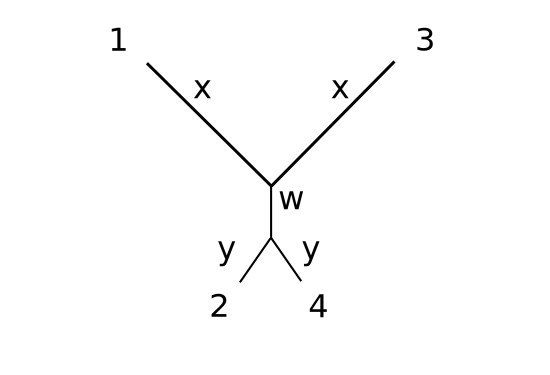
\includegraphics[width=.95\textwidth]{farris_blank}
\caption[short]{Farris topology $\tau_1$}
\end{subfigure}
\begin{subfigure}{.45\linewidth}
\centering
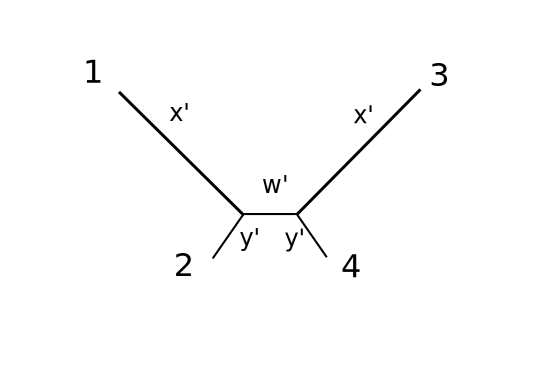
\includegraphics[width=.95\textwidth]{felsenstein_blank}
\caption[short]{Felsenstein topology $\tau_2$}
\end{subfigure}
\caption{Two simple topologies}
\label{fig:farris-fels-top}
\end{figure}

Define the Farris topology $\tau_1$ and the Felsenstein topology $\tau_2$ as in Figure~\ref{fig:farris-fels-top}.
Call $t=\{x,y,w\}$ and $t^*=\{x,y,y\}$, i.e., $t^*$ is the case where the bottom three branches all share the same parameter, the classical construction of this topology.
The branch length parameters are such that the probability of a change in character along the top two branches is $p_x=1-2x$, with corresponding equalities for the other two branches.
Here, $\{p_x,p_y,p_z\}\in[0,1/2]^3$ and $\{x,y,z\}\in[0,1]^3$.

\textbf{Justification for estimand:} It might be worth arguing why this form of the estimand $t$ is necessary.
I think the idea is that for either of these topologies, any maximum obtained will occur where the top two and bottom two branches are equal, though not necessarily the middle branch.
This would be good to show explicitly.

Table~\ref{tab:sitepatprob} contains calculations of site pattern frequencies under these two topologies, calculated using the Hadamard transform approach outlined in 8.6 of Semple and Steel \cite{Semple2003-em}.
Table~\ref{tab:likelihoods} contains calculations of likelihood values for fixed site patterns and topologies, with the maximum values over ancestral state patterns noted.

\begin{table}
\centering
\begin{tabular}{|l|l|l|}
\multicolumn{3}{c}{Classical}\\
    \hline
$s_j$   &$P(s_j|\tau_1,t^*)$&$P(s_j|\tau_2,t^*)$\\
    \hline
0000&$1+x^2+y^2+4xy^2+x^2y^2$&$1+2xy+2xy^2+x^2y+y^3+x^2y^2$\\
0001&$1+x^2-y^2-x^2y^2$&$1+x^2y-y^3-x^2y^2$\\
0010&$1-x^2+y^2-x^2y^2$&$1-x^2y+y^3-x^2y^2$\\
0100&$1+x^2-y^2-x^2y^2$&$1+x^2y-y^3-x^2y^2$\\
1000&$1-x^2+y^2-x^2y^2$&$1-x^2y+y^3-x^2y^2$\\
0011&$1-x^2-y^2+x^2y^2$&$1+2xy-2xy^2-x^2y-y^3+x^2y^2$\\
0101&$1+x^2+y^2-4xy^2+x^2y^2$&$1-2xy-2xy^2+x^2y+y^3+x^2y^2$\\
1001&$1-x^2-y^2+x^2y^2$&$1-2xy+2xy^2-x^2y-y^3+x^2y^2$\\
    \hline
\multicolumn{3}{c}{Modified}\\
    \hline
$s_j$   &$P(s_j|\tau_1,t)$&$P(s_j|\tau_2,t)$\\
    \hline
0000&$1+x^2+y^2+4xyw+x^2y^2$&$1+2xy+2xyw+x^2w+y^2w+x^2y^2$\\
0001&$1+x^2-y^2-x^2y^2$&$1+x^2w-y^2w-x^2y^2$\\
0010&$1-x^2+y^2-x^2y^2$&$1-x^2w+y^2w-x^2y^2$\\
0100&$1+x^2-y^2-x^2y^2$&$1+x^2w-y^2w-x^2y^2$\\
1000&$1-x^2+y^2-x^2y^2$&$1-x^2w+y^2w-x^2y^2$\\
0011&$1-x^2-y^2+x^2y^2$&$1+2xy-2xyw-x^2w-y^2w+x^2y^2$\\
0101&$1+x^2+y^2-4xyw+x^2y^2$&$1-2xy-2xyw+x^2w+y^2w+x^2y^2$\\
1001&$1-x^2-y^2+x^2y^2$&$1-2xy+2xyw-x^2w-y^2w+x^2y^2$\\
    \hline
\end{tabular}
\caption{Site pattern probabilities.
All values are multiplied by $1/8$.}
\label{tab:sitepatprob}
\end{table}

\begin{table}
\centering
\begin{tabular}{|l|ll|}
\multicolumn{3}{c}{$P(z_j|s_j,\tau_1,t)$}\\
\hline
& \multicolumn{2}{|c|}{$z_j$}\\
    \hline
$s_j$    &00                              &01\\
    \hline
0000&$(1+x)^2   (1+w)(1+y)^{2*}$          &$(1+x)^2   (1-w)(1-y)^2$\\
0001&$(1+x)^2   (1+w)(1+y)(1-y)^*$        &$(1+x)^2   (1-w)(1+y)(1-y)$\\
0010&$(1+x)^2   (1+w)(1+y)(1-y)^*$        &$(1+x)^2   (1-w)(1+y)(1-y)$\\
0100&$(1+x)(1-x)(1+w)(1+y)^{2*}$          &$(1+x)(1-x)(1-w)(1-y)^2$\\
1000&$(1+x)(1-x)(1+w)(1+y)^{2*}$          &$(1+x)(1-x)(1-w)(1-y)^2$\\
0011&$(1+x)(1-x)(1+w)(1+y)(1-y)^{\dagger}$&$(1+x)(1-x)(1-w)(1+y)(1-y)$\\
0101&$(1+x)^2   (1+w)(1-y)^{2\ddagger}$   &$(1+x)^2   (1-w)(1+y)^{2\ddagger}$\\
1001&$(1+x)(1-x)(1+w)(1+y)(1-y)^{\dagger}$&$(1+x)(1-x)(1-w)(1+y)(1-y)$\\
    \hline
    \hline
&10                           &11\\
    \hline
0000&$(1-x)^2   (1-w)(1+y)^2$     &$(1-x)^2   (1+w)(1-y)^2$\\
0001&$(1-x)^2   (1-w)(1+y)(1-y)$  &$(1-x)^2   (1+w)(1+y)(1-y)$\\
0010&$(1-x)^2   (1-w)(1+y)(1-y)$  &$(1-x)^2   (1+w)(1+y)(1-y)$\\
0100&$(1+x)(1-x)(1-w)(1+y)^2$     &$(1+x)(1-x)(1+w)(1-y)^2$\\
1000&$(1+x)(1-x)(1-w)(1+y)^2$     &$(1+x)(1-x)(1+w)(1-y)^2$\\
0011&$(1+x)(1-x)(1-w)(1+y)(1-y)$  &$(1+x)(1-x)(1+w)(1+y)(1-y)^{\dagger}$\\
0101&$(1-x)^2   (1-w)(1-y)^2$     &$(1-x)^2   (1+w)(1+y)^{2\ddagger}$\\
1001&$(1+x)(1-x)(1-w)(1+y)(1-y)$  &$(1+x)(1-x)(1+w)(1+y)(1-y)^{\dagger}$\\
    \hline
    \multicolumn{3}{c}{$P(z_j|s_j,\tau_2,t)$}\\
\hline
& \multicolumn{2}{|c|}{$z_j$}\\
    \hline
$s_j$    &00                              &01\\
    \hline
0000&$(1+x)^2   (1+w)(1+y)^{2*}$           &$(1+x)(1-x)(1-w)(1+y)(1-y)$\\
0001&$(1+x)^2   (1+w)(1+y)(1-y)^{\ddagger}$&$(1+x)(1-x)(1-w)(1+y)^{2\ddagger}$\\
0010&$(1+x)(1-x)(1+w)(1+y)^{2\ddagger}$    &$(1+x)^2   (1-w)(1+y)(1-y)^{\ddagger}$\\
0100&$(1+x)^2   (1+w)(1+y)(1-y)^{\ddagger}$&$(1+x)(1-x)(1-w)(1-y)^2$\\
1000&$(1+x)(1-x)(1+w)(1+y)^{2\ddagger}$    &$(1-x)^2   (1-w)(1+y)(1-y)$\\
0011&$(1+x)(1-x)(1+w)(1+y)(1-y)^{\ddagger}$&$(1+x)^2   (1-w)(1+y)^{2\ddagger}$\\
0101&$(1+x)^2   (1+w)(1-y)^{2\ddagger}$    &$(1+x)(1-x)(1-w)(1+y)(1-y)^{\ddagger}$\\
1001&$(1+x)(1-x)(1+w)(1+y)(1-y)^{\ddagger}$&$(1-x)^2   (1-w)(1+y)^{2\ddagger}$\\
    \hline
    \hline
&10                           &11\\
    \hline
0000&$(1+x)(1-x)(1-w)(1+y)(1-y)$             &$(1-x)^2   (1+w)(1-y)^2$\\
0001&$(1+x)(1-x)(1-w)(1-y)^2$                &$(1-x)^2   (1+w)(1+y)(1-y)$\\
0010&$(1-x)^2   (1-w)(1+y)(1-y)$             &$(1+x)(1-x)(1+w)(1-y)^2$\\
0100&$(1+x)(1-x)(1-w)(1+y)^{2\ddagger}$      &$(1-x)^2   (1+w)(1+y)(1-y)$\\
1000&$(1+x)^2   (1-w)(1+y)(1-y)^{\ddagger}$  &$(1+x)(1-x)(1+w)(1-y)^2$\\
0011&$(1-x)^2   (1-w)(1-y)^2$                &$(1+x)(1-x)(1+w)(1+y)(1-y)^{\ddagger}$\\
0101&$(1+x)(1-x)(1-w)(1+y)(1-y)^{\ddagger}$  &$(1-x)^2   (1+w)(1+y)^{2\ddagger}$\\
1001&$(1+x)^2   (1-w)(1-y)^{2\ddagger}$      &$(1+x)(1-x)(1+w)(1+y)(1-y)^{\ddagger}$\\
\hline
\end{tabular}
\caption{Likelihood calculations for all site patterns and internal states of Farris topology.
Maxima determined row-wise (i.e., by site pattern).
All values multiplied by $1/32$.
Key: $^*$ unique maximum value corresponding to unique internal state; $^\dagger$ unique maximum value corresponding to multiple internal states; $^\ddagger$ multiple maximum values corresponding to multiple internal states.}
\label{tab:likelihoods}
\end{table}

\subsection{Bounding the likelihoods}

Assume $\tau^*=\tau_1$ and $t^*=\{x,y,y\}$.
Our approach will be to decompose the likelihood inside the maximization in \eqref{eq:site_pattern_profile_likelihood_mean} as
\begin{equation}
\label{eq:partial-likelihood}
L(x', y', w'; \mathbf{z},\tau') = H(x,y,\tau_1;x',y',w', \tau') + L_{p}(x',y',w';\mathbf{z},\tau')
\end{equation}
where different values for $\mathbf{z}$ will alter the form of $L_{p}(x',y',w';\mathbf{z},\tau')$.
We obtain an upper bound for the joint maximum of \eqref{eq:partial-likelihood}
$$
\max_{\{x',y',w',\mathbf{z}\}} \ L(x',y',w';\mathbf{z},\tau') \le H(x,y,\tau_1;x,y,y,\tau_1) + L_{p}(\hat{x}, \hat{y}, \hat{w};\hat{\mathbf{z}},\tau')
$$
using Gibbs inequality
$$
H(x, y, \tau_1;x', y', w', \tau') \le H(x, y, \tau_1;x, y, y, \tau_1)
$$
and
$$
\{\hat{x}, \hat{y}, \hat{w}, \hat{\mathbf{z}}\} = \arg\max_{\{x,y,w,\mathbf{z}\}} \ L_{p}(x,y,w;\mathbf{z},\tau').
$$
Similarly, we have a lower bound as
$$
\max_{\{x',y',w',\mathbf{z}\}} \ L(x',y',w';\mathbf{z},\tau') \ge H(x,y,\tau_1; \hat{x}, \hat{y}, \hat{w}, \tau') + L_{p}(\hat{x}, \hat{y}, \hat{w},\hat{\mathbf{z}},\tau').
$$

% vvvv Remove these? I think they're obvious now, but maybe they can be made more explicit above?
\textbf{Argument for lower bound}: This makes intuitive sense, though may be difficult to show in general.
Can we not just say $\max_u f(u) + g(u)$ is greater than $f(u') + g(u')$ for any $u'$ that doesn't maximize $f(u) + g(u)$ just by definition?
There could be multiple maxima, but that's why we have greater than or equal to.
I think the only thing we'd need to show is that a maximum exists, but since $\{x,y,w\}$ are supported on a closed set this is certainly true.
I must be missing something.

\textbf{Argument for upper bound}: I think this is true mostly because $\max_u f(u) + g(u)$ should be less than $\max_u f(u) + \max_u g(u)$ by some triangle inequality argument.
If we were to actually maximize the full likelihood, we should get something smaller than maximizing some form of it that we consider by looking at the parts separately.
For a fixed $\{x^*, y^*\}$ we can calculate this upper bound directly---can we obtain it as a useful-looking function of these parameters in the general case?

\subsubsection{Upper bound for Farris likelihood}

To obtain an upper bound for the Farris likelihood---the terms in the top half of Table~\ref{tab:likelihoods}---we use the term $(1+x)^2(1+w)(1+y)^2$ for the $0101$ site pattern.
Since all cases have a $(1+x)^2$ term except $\{0100, 1000, 0011, 1001\}$, and all cases except $\{0001, 0010, 0011, 1001\}$ have a $(1+y)^2$, we can add and subtract the $\log$ of these terms weighted by each of their generating probabilities.
In other words, define
$$
a = P(0100|\tau_1,\{x,y,y\}) + P(1000|\tau_1,\{x,y,y\}) + P(0011|\tau_1,\{x,y,y\}) + P(1001|\tau_1,\{x,y,y\})
$$
and
$$
b = P(1000|\tau_1,\{x,y,y\}) + P(0010|\tau_1,\{x,y,y\}) + P(0011|\tau_1,\{x,y,y\}) + P(1001|\tau_1,\{x,y,y\}).
$$
Then the ancestral state maximizing the likelihood is $00$ and $L_{p}(x',y',w';\mathbf{z},\tau_1)$ is bounded above by
$$
L_{p}(x',y',w';00,\tau_1) \le (2-a)\log(1+x')+a\log(1-x')+(2-b)\log(1+y')+b\log(1-y')+\log(1+w')
$$
with a maximum
$$
\hat{L}_{p}(1-a,1-b,1;00,\tau_1) \le (2-a)\log(2-a)+a\log(a)+(2-b)\log(2-b)+b\log(b)+\log(2)
$$
where $a$ and $b$ are functions of the true generating branch parameters $\{x,y\}$.

\subsubsection{Lower bound for Felsenstein likelihood}

We construct a similar lower bound on the Felsenstein likelihood, though here we replace all $(1+w)$ terms with $(1-w)$.
Let
$$
c = P(0001|\tau_1,\{x,y,y\}) + P(0010|\tau_1,\{x,y,y\}) + P(0100|\tau_1,\{x,y,y\}) + P(1000|\tau_1,\{x,y,y\})
$$
and
$$
d = P(0101|\tau_1,\{x,y,y\}) + P(1001|\tau_1,\{x,y,y\}).
$$
The lower bounds on the likelihoods in this case take one of six forms:
\textbf{TODO}: ancestral states where these likelihoods occur
$$
L_{p}(x',y',w';z,\tau_2) \ge 2\log(1+x')+(2-c-2d)\log(1+y')+(c+2d)\log(1-y')+\log(1-w'),
$$
$$
L_{p}(x',y',w';z,\tau_2) \ge (2-c-2d)\log(1+x')+(c+2d)\log(1-x')+2\log(1+y')+\log(1-w'),
$$
$$
L_{p}(x',y',w';z,\tau_2) \ge (2-2d)\log(1+x')+2d\log(1-x')+(2-c)\log(1+y')+c\log(1-y')+\log(1-w'),
$$
$$
L_{p}(x',y',w';z,\tau_2) \ge (2-c)\log(1+x')+c\log(1-x')+(2-2d)\log(1+y')+2d\log(1-y')+\log(1-w'),
$$
$$
L_{p}(x',y',w';z,\tau_2) \ge (2-d)\log(1+x')+d\log(1-x')+(2-c-d)\log(1+y')+(c+d)\log(1-y')+\log(1-w')
$$
or
$$
L_{p}(x',y',w';z,\tau_2) \ge (2-c-d)\log(1+x')+(c+d)\log(1-x')+(2-d)\log(1+y')+d\log(1-y')+\log(1-w').
$$
Since the maxima for pairs of lower bounds above each have a symmetry in $x$ and $y$, they are bounded below by one of
$$
\hat{L}_{p}(1,1-c-2d,0;z,\tau_2) \ge 2\log(2)+(2-c-2d)\log(2-c-2d)+(c+2d)\log(c+2d),
$$
$$
\hat{L}_{p}(1-2d,1-c,0;z,\tau_2) \ge (2-2d)\log(2-2d)+2d\log(2d)+(2-c)\log(2-c)+c\log(c)
$$
and
$$
\hat{L}_{p}(1-d,1-c-d,0;z,\tau_2) \ge (2-d)\log(2-d)+d\log(d)+(2-c-d)\log(2-c-d)+(c+d)\log(c+d)
$$
where $c$ and $d$ are also functions of the true generating branch parameters $\{x,y\}$.

\textbf{TODO}: cases for $\{x, y\}$ where each of the above is the corresponding maximum.
I think the first is always greater than or equal to the other two, but I haven't been able to show it yet.
It may take a little information theory--fu, or just standard application of the bounds in the introduction to this section.

Thus, let
$$
\hat{L}_{p}(1,1-c-2d,0;z,\tau_2) = 2\log(2)+(2-c-2d)\log(2-c-2d)+(c+2d)\log(c+2d).
$$

\subsubsection{Region of inconsistency}

We want to find values for $\{x,y\}$ where
$$
H(x,y,\tau_1; 1, 1-c-2d, 0, \tau_2) + \hat{L}_{p}(1,1-c-2d,0;z,\tau_2) \ge H(x,y,\tau_1; x, y, y,\tau_1) + \hat{L}_{p}(1-a,1-b,1;00,\tau_1).
$$
Since this is a single inequality in two variables, we can plot it analytically; we need the region where
\begin{align*}
    0 &\ge H(x,y,\tau_1; x, y, y,\tau_1) + \hat{L}_{p}(1-a,1-b,1;00,\tau_1) \\
      &\qquad - H(x,y,\tau_1; 1, 1-c-2d, 0, \tau_2) - \hat{L}_{p}(1,1-c-2d,0;\tau_2) \\
      & = 2(12+2x^2+2y^2)\log((12+2x^2+2y^2)/8) \\
      &\qquad + 2(4-2x^2-2y^2)\log((4-2x^2-2y^2)/8)  + 8\log2 \\
      &\qquad + 2(1+x^2-y^2-x^2y^2)\log(1+x^2-y^2-x^2y^2) \\
      &\qquad + 2(1-x^2+y^2-x^2y^2)\log(1-x^2+y^2-x^2y^2) \\
      &\qquad + 2(1-x^2-y^2+x^2y^2)\log(1-x^2-y^2+x^2y^2) \\
      &\qquad + (1+x^2+y^2+4xy^2+x^2y^2)\log(1+x^2+y^2+4xy^2+x^2y^2) \\
      &\qquad + (1+x^2+y^2-4xy^2+x^2y^2)\log(1+x^2+y^2-4xy^2+x^2y^2) \\
      &\qquad - 16\log2 - 8(1+xy^2)\log(1+xy^2) - 8(1-xy^2)\log(1-xy^2) \\
      &\qquad - (2-4xy^2+2x^2y^2)\log(1-2xy^2+x^2y^4) \\
      &\qquad - (2+4xy^2+2x^2y^2)\log(1+2xy^2+x^2y^4) \\
      &\qquad - (4-4x^2y^2)\log(1-x^2y^4).
\end{align*}

\textbf{TODO}: can we use sage to simplify the above so it looks nicer?
Write it as functions of $a,b,c,d$ so it's less messy?
What would be best?

The \texttt{sage} function in listing~\ref{list:sage} will generate Fig.~\ref{fig:inconsistency-farris}.

\begin{table}
    \begin{center}
\begin{verbatim}
var('x,y')
inconsistency = 2*(12+2*x^2+2*y^2)*log((12+2*x^2+2*y^2)/8) \
    + 2*(4-2*x^2-2*y^2)*log((4-2*x^2-2*y^2)/8) + 8*log(2.) \
    + 2*(1+x^2-y^2-x^2*y^2)*log(1+x^2-y^2-x^2*y^2) \
    + 2*(1-x^2+y^2-x^2*y^2)*log(1-x^2+y^2-x^2*y^2) \
    + 2*(1-x^2-y^2+x^2*y^2)*log(1-x^2-y^2+x^2*y^2) \
    + (1+x^2+y^2+4*x*y^2+x^2*y^2)*log(1+x^2+y^2+4*x*y^2+x^2*y^2) \
    + (1+x^2+y^2-4*x*y^2+x^2*y^2)*log(1+x^2+y^2-4*x*y^2+x^2*y^2) \
    - 16*log(2.) - 8*(1+x*y^2)*log(1+x*y^2) - 8*(1-x*y^2)*log(1-x*y^2) \
    - (2-4*x*y^2+2*x^2*y^2)*log(1-2*x*y^2+x^2*y^4) \
    - (2+4*x*y^2+2*x^2*y^2)*log(1+2*x*y^2+x^2*y^4) - (4-4*x^2*y^2)*log(1-x^2*y^4)

inconsistency_plot = implicit_plot(
    inconsistency(x,y)==0,
    (x,0,1),
    (y,0,1),
    axes_labels=['$x$', '$y$'],
    title='Region of inconsistency for Farris-generating topology',
    color='black'
)
\end{verbatim}
    \end{center}
\caption{Sage code to generate Fig.~\ref{fig:inconsistency-farris}}
\label{list:sage}
\end{table}

\begin{figure}
\centering
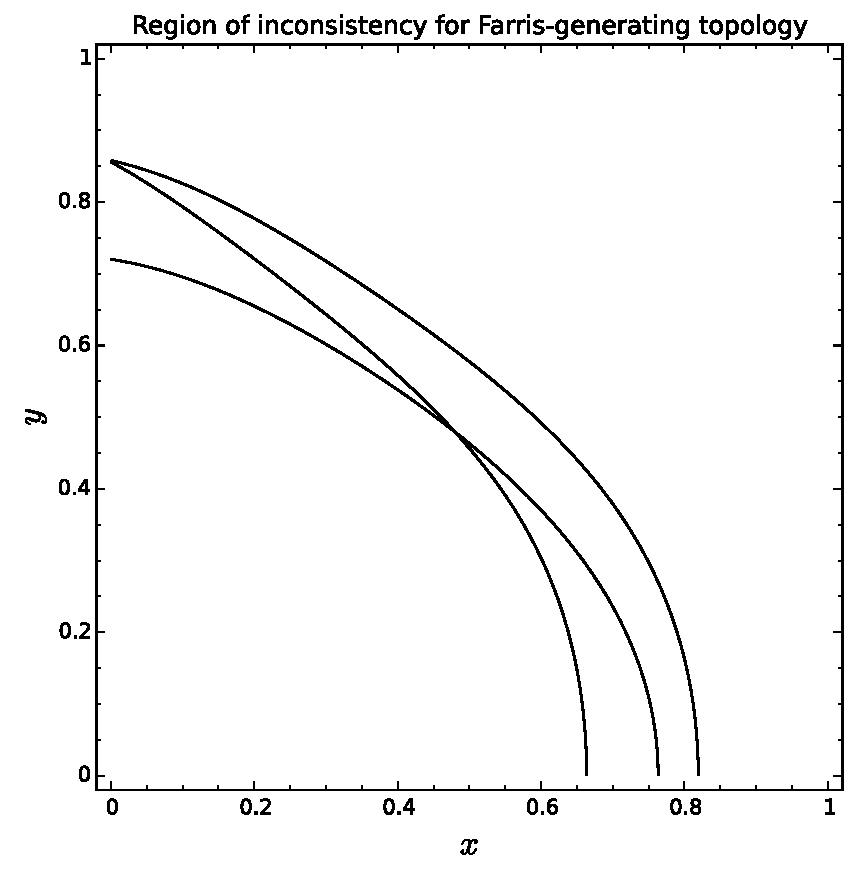
\includegraphics[width=.9\textwidth]{analytic-inconsistency}
\caption{Regions of inconsistency}
\label{fig:inconsistency-farris}
\end{figure}

\paragraph{Example}

Set $\{x, y\} = \{0.25, 0.25\}$.
For a Farris zone generating topology, we have
$$
a = b = 0.46875
$$
resulting in
$$
\hat{L}^{p}(\hat{x}, \hat{y}, \hat{w},\tau_1) \approx -2.17803560694
$$
and
$$
H(x,y,\tau_1;x,y,y,\tau_1) \approx -2.07509999739.
$$
Computing the upper bound yields
$$
\max_{x,y,w} \ L(x,y,w,\tau_1) \le -4.25313560433
$$
and it remains to show that
$$
\max_{x,y,w} \ L(x,y,w,\tau_2) \ge -4.25313560433
$$

For the same generating parameters,
$$
c = 0.498046875, \ d = 0.2431640625,
$$
resulting in
$$
\hat{L}(\hat{x}, \hat{y}, \hat{w},\tau_2) \approx -2.07919739112
$$
Calculating shows%
    %
    \footnote{It's not a typo that $\hat{L}_{fe}$ and $H_{fe}$ are the same---at least not in the code.
        I should try to show why this is the case.
        }
    %
$$
H(x,y,\tau_1; \hat{x}, \hat{y}, \hat{w},\tau_2) \approx -2.07919739112
$$
and
$$
\max_{x,y,w} \ L(x,y,w,\tau_2) \ge -4.15839478224 > -4.25313560433 \ge \max_{x,y,w} \ L(x,y,w,\tau_1)
$$
where site patterns are generated from the Farris zone topology.
Confirming, run \texttt{python}'s numerical optimization solver for $\{.25, .25\}$.
Since we are computing a constrained maximization, we can find a global maximum using basin hopping, and doing so yields
$$
\max_{x,y,w} \ L(x,y,w,\tau_1) \approx -4.5101771294218045
$$
and
$$
\max_{x,y,w} \ L(x,y,w,\tau_2) \approx -4.1544859851260281.
$$
Woohoo!



\section{Discussion}

Neyman-Scott paradox.

Interesting that here we are simulating on the Farris tree and end up with the Felsenstein tree.
For maximum parsimony it's the opposite \cite{Felsenstein1978-rr}.
Discussion of number of parameters of each.

However, note that \cite{Siddall1998-hq} get things going the same way, although \cite{Swofford2001-hr} show that the problem is that they didn't simulate long enough sequences.

\bibliographystyle{plain}
\bibliography{joint_inf}

\end{document}
